% see A1.1a
\chapter{Informieren}

Die nachfolgende Dokumentation baut auf der Vorlage \cite{Buhler_ipa-template_2022} auf.

\section{Projektmanagement}

Das Projekt wird nach der Projektmanagementmethode IPERKA abgewickelt. Diese Methode passt zum Auftrag, weil der Auftrag in einer Iteration innerhalb von 10 Tagen wasserfallartig realisiert werden soll.

\subsection{Arbeitspakete}

Der Auftrag kann in folgende Arbeitspakete aufgeteilt und nach den Phasen der Projektmanagementmethode gegliedert werden:

\begin{itemize}
    \item Informieren
    \begin{description}
        \item[AP1: Anforderungen analysieren] Der Auftrag wird analysiert und daraus einzelne Arbeitspakete abgeleitet. 
        \item[AP2: Kurzfassung ableiten und schreiben] Es wird anhand der Analyse eine Kurzfassung des Auftrages abgeleitet und verfasst.
        \item[AP3: Firmenstandards] Die Firmenstandards werden dokumentiert.
    \end{description}
    \item Planen
    \begin{description}
        \item[AP4: Zeitplan gestalten] Es wird anhand der Arbeitspakete ein Zeitplan gestaltet.
        \item[AP5: Gestalten von Diagrammen] Verschiedene Diagramme werden für die bildliche Darstellung des Systemes gestaltet.
        \item[AP6: Testkonzept] Testfälle sowie verschiedene Arten zu testen werden festgehalten und genau dokumentiert.
    \end{description}
    \item Entscheiden
    \begin{description}
        \item[AP7: Bewerten von verschiedenen Optionen] Alle möglichen Optionen werden (falls es eine Entscheidung zum Treffen gibt) ausgewertet. Die Auswertemethode kann je nach Anwendungsfall verschieden sein.
        \item[AP6: Entscheiden der Optionen] Nach der Auswertung, wird eine der Optionen genommen. Dies wird dokumentiert.
    \end{description}
    \item Realisieren
    \begin{description}
        \item[AP7: Aufsetzen des Projektes] Das Projekt wird aufgesetzt und mit GitHub verbunden. Das Gleiche gilt für die CI. \newline
        Es werden auch die nötigen \gls{Hooks} auf allen nötigen Diensten eingestellt.
        \item[AP10: Umsetzen der Datenstruktur auf Basis der Diagramme] Die Datenstruktur wird im Projekt umgesetzt. Diese soll nicht von den Diagrammen abweichen.
        \item[AP11: Daten erstellen und manipulieren] Das erstellen, sowie Manipulieren von Daten anhand der Webhooks soll umgesetzt werden.
        \item[AP12: Implementieren der \gls{Business-Logic}] Die Business Logic wird implementiert. Damit ist das Auswerten der Daten gemeint.
        \item[AP13: Erstellen der \gls{Views}] Die Views werden anhand der \gls{Mockups} erstellt.
    \end{description}
    \item Kontrollieren
    \begin{description}
        \item[AP14: Nach Testkonzept testen] Das Testkonzept wird als Checkliste verwendet und die einzelnen Tests werden nach Protokoll durchgeführt \newline
        Das individuelle Kriterium 7 (Automatisierte Tests) wird auch dokumentiert.
        \item[AP15: Kopplung vom Hauptprogramm] In Retrospektive wird festgehalten wie gut das Programm vom Hauptprogramm abgekoppelt ist.
    \end{description}
    \item Auswerten
    \begin{description}
        \item[AP16: Auswerten] Es wird eine Auswertung beziehungsweise Reflexion über das Projekt geschrieben.
    \end{description}
\end{itemize}

\section{Systemaufbau}
Im Folgenden wird die Einbettung des Systems in das Gesamtsystem gezeigt, sowie die vorhandenen Schnittstellen und Akteure beschrieben.

\begin{minipage}{\textwidth}
    \subsection{Gesamtsystem}
    Das Gesamtsystem wird hier anhand eines Deployment-Diagramms dargestellt. Dieses zeigt die einzelnen Komponenten und deren Verbindungen.
    \begin{center}
        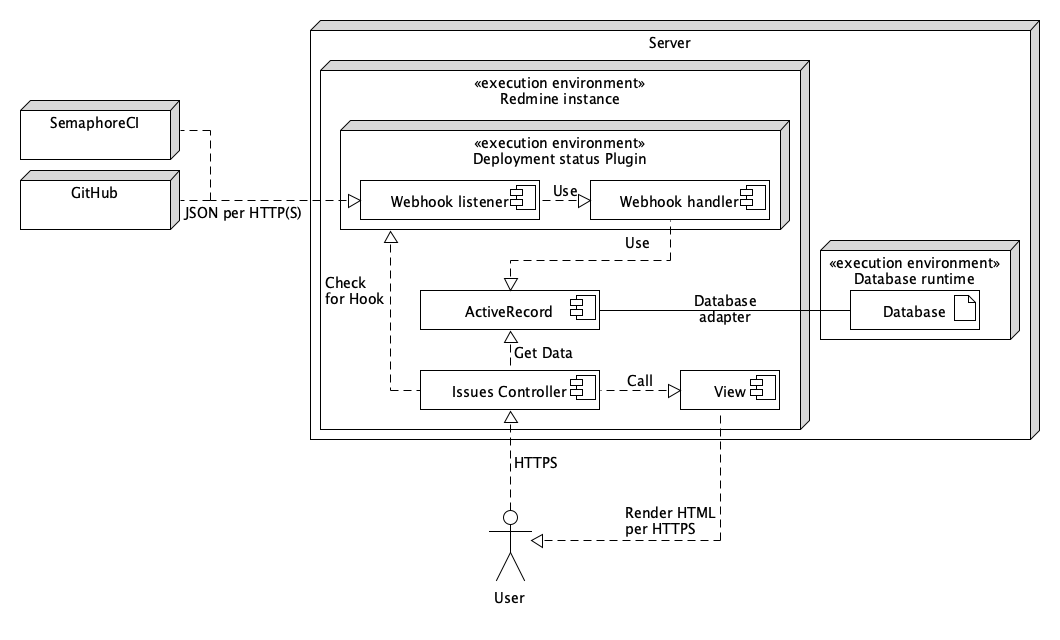
\includegraphics[width=0.8\textwidth]{images/deployment-diagram.png}
        \label{fig:deployment-diagram}
    \end{center}
\end{minipage}

\subsection{Schnittstellen}
Dieses Kapitel beschreibt die in der Grafik \ref{fig:deployment-diagram} gezeigten Schnittstellen im Detail.
Unter Schnittstellen gelten Elemente, die ausserhalb des Plugins liegen.

\subsubsection{SemaphoreCI}
SemaphoreCI ist ein Dienst, welcher die CI/CD Pipeline für Projekte bereitstellt. Dieser hat ein
\enquote{Notification} System, welches bei bestimmten Events (in diesem Fall Deployments) JSON Daten
an eine URL sendet. In diesem Fall wird die URL vom Plugin bereitgestellt.

\subsubsection{GitHub}
GitHub ist ein Dienst, welcher die Versionsverwaltung für Projekte bereitstellt. Dieser hat, gleich wie
SemaphoreCI, ein System, welches JSON Daten bei bestimmten Events verschickt. Der Unterschied hier ist, dass
diese Daten das Plugin bei einer Pull Request erreichen, anstatt bei einem Deployment.

\subsubsection{Database}
Die Database repräsentiert die Datenbank, welche von der Redmine-Instanz verwendet wird. Diese kann dank
Redmine (fast) jedes beliebige Datenbanksystem sein. In der Regel wird bei der Renuo AG PostgreSQL verwendet.

\subsubsection{ActiveRecord}
ActiveRecord ist ein ORM (Object Relational Mapping) für Ruby. Dieses stellt eine Schnittstelle zwischen der
Datenbank und dem Rails Programm dar. Es wird verwendet, um die Datenbank zu abstrahieren und die Daten
in Objekte zu konvertieren.

\subsection{Issues Controller}
Der Issues Controller ist der von Redmine bereits vorhandene Controller, welcher für die Issues zuständig ist.
Er kümmert sich um die Auflistung sowie detailierte Ansicht für Issues. Dieser Controller steht im System
verbunden mit einem \enquote{Check for Hook} mit dem Plugin in Verbindung. Das bedeutet, dass das Plugin die
Funktionalität des Controllers erweitert.

\subsection{View}
Die View ist das zurückgeschickte HTML vom Controller.

\subsection{Akteure}
\begin{tabularx}{\textwidth}[H]{|c|X|}
  \hline
  User & Der \enquote{User} ist der Redmine-Nutzer. Dieser kann eine beliebige Rolle haben, solange er die 
  Issues lesen darf. \\ \hline
  GitHub \& SemaphoreCI & Diese beiden Akteure sind die Dienste, welche auf die Schnittstellen zugreifen.
  \\ \hline
\end{tabularx}
